\documentclass[10pt,letterpaper]{article}
\usepackage[top=0.85in,left=2.75in,footskip=0.75in]{geometry}

% amsmath and amssymb packages, useful for mathematical formulas and symbols
\usepackage{amsmath,amssymb}

% Use adjustwidth environment to exceed column width (see example table in text)
\usepackage{changepage}

% Use Unicode characters when possible
\usepackage[utf8x]{inputenc}

% textcomp package and marvosym package for additional characters
\usepackage{textcomp,marvosym}

% cite package, to clean up citations in the main text. Do not remove.
\usepackage{cite}

% Use nameref to cite supporting information files (see Supporting Information section for more info)
\usepackage{nameref,hyperref}

% line numbers
\usepackage[right]{lineno}

% ligatures disabled
\usepackage{microtype}
\DisableLigatures[f]{encoding = *, family = * }

% color can be used to apply background shading to table cells only
\usepackage[table]{xcolor}

% array package and thick rules for tables
\usepackage{array}

% enumerate package lets us use letters instead of numbers
\usepackage{enumerate}

% create "+" rule type for thick vertical lines
\newcolumntype{+}{!{\vrule width 2pt}}

% create \thickcline for thick horizontal lines of variable length
\newlength\savedwidth
\newcommand\thickcline[1]{%
  \noalign{\global\savedwidth\arrayrulewidth\global\arrayrulewidth 2pt}%
  \cline{#1}%
  \noalign{\vskip\arrayrulewidth}%
  \noalign{\global\arrayrulewidth\savedwidth}%
}

% \thickhline command for thick horizontal lines that span the table
\newcommand\thickhline{\noalign{\global\savedwidth\arrayrulewidth\global\arrayrulewidth 2pt}%
\hline
\noalign{\global\arrayrulewidth\savedwidth}}

\usepackage{color}

% Remove comment for double spacing
%\usepackage{setspace}
%\doublespacing

% Text layout
\raggedright
\setlength{\parindent}{0.5cm}
\textwidth 5.25in
\textheight 8.75in

% Bold the 'Figure #' in the caption and separate it from the title/caption with a period
% Captions will be left justified
\usepackage[aboveskip=1pt,labelfont=bf,labelsep=period,justification=raggedright,singlelinecheck=off]{caption}
\renewcommand{\figurename}{Fig}

% Use the PLoS provided BiBTeX style
\bibliographystyle{plos2015}

% Remove brackets from numbering in List of References
\makeatletter
\renewcommand{\@biblabel}[1]{\quad#1.}
\makeatother

% Leave date blank
\date{}

% Header and Footer with logo
\usepackage{lastpage,fancyhdr,graphicx}
\usepackage{epstopdf}
\pagestyle{myheadings}
\pagestyle{fancy}
\fancyhf{}
\setlength{\headheight}{27.023pt}
\lhead{
\includegraphics[width=2.0in]{PLOS-submission.eps}}
\rfoot{\thepage/\pageref{LastPage}}
\renewcommand{\footrule}{\hrule height 2pt \vspace{2mm}}
\fancyheadoffset[L]{2.25in}
\fancyfootoffset[L]{2.25in}
\lfoot{\sf PLOS}


%% Define per-paper macros.
\newcommand{\rulemajor}[1]{\section{#1}}
\begin{document}
\vspace*{0.2in}

\begin{flushleft}
{\Large
\textbf\newline{Ten Simple Rules for Thinking Like a Programmer}
}
\newline
\\
{Greg~Wilson}\textsuperscript{1,*}
\\
\textbf{1} RStudio, Inc. / greg.wilson@rstudio.com
\\
\bigskip
* Corresponding author.
\end{flushleft}

\section*{Abstract}

We describe ten characteristic ways in which programmers view the world that are
often useful in other contexts.

\section*{Author Summary}

The term ``computational thinking'' is widely used, but there is little
consensus on what it actually encompasses.  Experienced programmers, on the
other hand, tend to think about problems in similar ways, and understanding
these ways can help people in other domains see their own fields with fresh
eyes.

\section*{Introduction}

The term ``computational thinking'' has been widely used since \cite{Wing2006}
introduced it more than a decade ago.  However, there is little consensus on
what it actually encompasses.  Experienced programmers, on the other hand,
tend to think about problems in similar ways, and understanding those ways
can help people in other domains---such as scientific research---see their
own fields with fresh eyes.

\subsection*{Acknowledgments}

An early version of this paper was inspired by Jon Udell's essay ``Seven Ways to
Think Like the Web'' \cite{Udel2011}.

\rulemajor{Programs are data.}

First, and most importantly, everything a computer works with is just 1's and
0's.  From email messages to pictures of far-off galaxies, it's all just bits.

This seems obvious, but one of its implications is that programs are just
another kind of data.  This is the key insight that all of modern computing is
built on.  The source code for a program is just a set of text files, no
different from a thesis or a poem.  Once that text is loaded into memory, the
instructions are just more bytes, and can be stored in data structures, passed
around, or altered.  Almost all advanced programming techniques, from callbacks
in JavaScript to decorators in Python and lazy evaluation in R, depend on this
fact in one way or another.

\rulemajor{Data must be interpreted.}

The complement to the first rule is that data doesn't mean anything on its
own---it has to be interpreted.  The bits 01100100011000010111100001100001 are
simultaneously the word ``data'', the integer 1,684,108,385, the floating-point
number 1.6635613602263159e+22, a bluish-gray pixel that's slightly transparent,
a medium-loud sound sample with slightly higher volume in the left channel, and
an instruction to multiply the value on the top of the stack by the value
beneath it and store the result in a particular location in memory.

A corollary is that machines don't understand: they only obey.  If you look at
this image, you see the word ``data'':


\includegraphics[width=5.0cm]{data.png}

A machine doesn't; it doesn't even see four blobs of blue pixels on a gray
background, because it doesn't ``see'' anything.  The computer stores this
image, and a program, as bits in memory.  If those bits happen to correspond to
instructions for the computer's CPU, and if those instructions happen to make up
a program for detecting shapes in images and matching those shapes with letters
in the alphabet, then the computer may very well output ``data'', but \emph{it
  doesn't understand}.  Calling a variable ``temperature'' doesn't mean the
computer will store a temperature in it---it would do exactly the same thing if
the variable was called ``pressure'' or ``frankenstein'' or ``a7''.  Again, this
may seem obvious, but thirty years after Pea first called it the ``superbug'',
believing that the computer will somehow understand intent remains a common
error \cite{Pea1986}.

\rulemajor{Programming is about creating and composing abstractions.}

Computers don't have to understand instructions in order to execute them, but we
need to understand them in order to create them (and fix them afterward).  Our
brains can only keep track of a handful of things at once \cite{Mill1956}, we
have to decompose complexity into chunks, then think in terms of those chunks.

One key to making abstraction work is to separate \emph{interface} and
\emph{implementation}.  An interface is what something knows how to do: the
questions it can answer, or the operations it can carry out. Its implementation
is how it does those things: what data it stores, what algorithms it uses, and
so on.  There can be dozens of ways to implement a particular interface; if we
do our work well, we shouldn't have to care about the implementation until
something goes wrong or we need to improve its performance.  ``Spare me the
details'' may be rude in real life, but it's essential in programming.

One useful rule of thumb is that every pattern is an abstraction trying to be
born.  Does your program repeatedly search an array to find the largest and
smallest values?  Write a function called \texttt{bounds}.  Does it repeatedly
search arbitrary data structures to find values that meet certain criteria?
Write a generator that returns values one by one and another function that
filters those according to some criteria.  The history of programming is in
large part the history of people noticing patterns and then making it easier
for programmers to work with them.

\rulemajor{Models are for computers, and views are for people.}

Another implication of the abstraction rule is important enough to be its own
rule: create models for computers and views for people.  A \emph{model} is a
representation of something that is easy for a computer to operate on; a
\emph{view} is a way of displaying it that human beings can understand.  For
example, an HTML page consists of elements that have attributes and that contain
other elements or blocks of text:

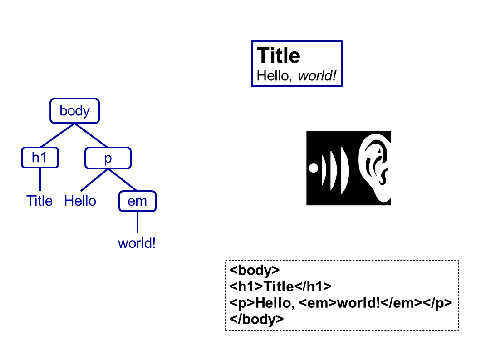
\includegraphics[width=10.0cm]{modelview.png}

That model can be rendered in a browser, turned into speech for someone who is
visually impaired, or displayed as text using angle brackets, quotes, and some
indentation.  None of these \emph{is} the model: they're all views that make the
model's content accessible to human beings in different contexts.  The model
itself isn't just easier for the computer to work with: it's essential, since as
we said before, the computer can't ``see'' the views that we create for human
beings.

Turning a view back into a model is hard: parsing the textual representation of
HTML takes thousands of lines of code, and doing OCR or speech recognition to
translate the rendered page or its spoken equivalent can take millions.  What
this idea implies, therefore, is that \emph{structured data is better than
  unstructured data}.  The tags and attributes in the textual representation of
an HTML page are there because without it, the computer can't tell whether
something is in italics because it's being emphasized or because it's the title
of a book.  To borrow an example from Jon Udell, a PDF with a cartoon whose
caption says, ``The knitting circle meets on the second Tuesday of every month''
is a lot easier for human beings to understand than a calendar entry in iCal
format, but the second is much easier for the computer.

\rulemajor{Paranoia makes us productive.}

Even simple software can go wrong in a bewildering variety of ways.  Since
fixing something after it breaks takes more time than getting it right in the
first place, experienced programmers have learned the value of investing time up
front in figuring out exactly what they're trying to accomplish, and in ensuring
that what they've built meets those requirements.  ``I want to count the stars
in this photograph'' is easy to say, but what does it actually mean?  What
constitutes a star?  When do you decide that a lumpy blob of pixels is two stars
rather than one, or three instead of two?  Every program embodies decisions
about questions like these, even if you don't realize that there was a question
and that you made a choice.

The sooner these decisions are made explicit and the earlier they're checked,
the less time is wasted.  Recent research shows that fine-grained
development---i.e., interleaving short bursts of coding and testing---is more
effective than working in larger chunks \cite{Fucc2017}, since the objectives
and implementation of the code are fresh in the programmer's mind while testing.

Of course, we don't stop worrying once we've typed our code in.  We check that
data is formatted properly to protect ourselves against ``garbage in, garbage
out''.  We put checks in our code to make sure that parameters are sensible,
data structures consistent, files aren't empty, and so on.  This is called
\emph{defensive programming}, and one of the signs of a mature programmer is
a high density of assertions and other self-checks in her code.

\rulemajor{Better algorithms are better than better hardware.}

One of the greatest mathematical advances of the Twentieth Century was the idea
of \emph{algorithmic complexity}, and its practical implications shape
everything we do with computers, whether we realize it or not.  The basic idea
is that we can estimate how the running time or memory requirements of an
algorithm grow as a function of the size of the problem we're trying to solve
\cite{Cone2016}.  while some algorithms slow down gently as their inputs get
larger, others slow down so much that even if the whole universe was one large
computer, it couldn't solve any problem big enough to be interesting.  Faster
chips help---a lot---but the real key to speed is to focus on how we're doing
things, not what we're doing it with.

But algorithms are nothing without data structures to operate on, just as data
structures are pointless without algorithms to manipulate them.  That's why the
two topics are usually taught together: arrays with loops, trees with recursion,
and so on.  Knowing the syntax of this language or the API of that library is
useful, but good programmers know their data structures and algorithms the way a
plumber knows pipes or a musician knows scales.

\rulemajor{Keep your bits close, and your frequently-used bits closer.}

FIXME: rule about locality and caching; refer back to pass-by-reference for the
web.  In particular, they know how to trade space for time and vice versa
\cite{Bent1982}.
  
\rulemajor{We can't break what we don't change.}

FIXME: rule 6 about immutable data structures being easier to understand; also
refer to library re-use (code is just data); include discussion of
pass-by-reference and pass-by-value.

Applies to workflows

One of the most effective ways to apply this principle is to automate
everything.  As Whitehead said \cite{Whit1958}, ``Civilization advances by
extending the number of important operations which we can perform without
thinking about them.''  Every time we automate a task, such as recompiling
software or re-running a data analysis when new input files appear, we reduce
the chances of getting it wrong the next time, and have more time to think about
things that machines \emph{can't} do for us.

\rulemajor{The street finds its own uses for things.}

The second rule is that every decision about what data to collect, who to share
it with, how to interpret it, and how to use those interpretations necessarily
and unavoidably furthers someone's interests.

FIXME: CITE Gibson ``Burning Chrome'' \cite{Gibs1987}

\rulemajor{The tool shapes the hand.}

Our final rule is something that artisans have known for thousands of years:
\emph{the tool shapes the hand}.  Building software changes how you use
software; making computers do new things changes your understanding of what
computers can do.  That's why the only way to learn how to think like a
programmer is to do some programming: however frustrating it may sometimes be,
it's the only way to learn what software can do for you, and how it can change
your view of everything else you do.

\bibliography{rules}

\end{document}
